\chapter{Logistic Regression and Optimizer}
Making a step back to the basics, we are given a training set $\{(X_i, Y_i)\}_{i=1}^N$, with $X_i \in \mathbb{R}^m$ and $Y_i \in \{0,1\}$ for all $i = 1, \dots, N$. Where:
\begin{compactitemize}
    \item $N$ is the number of training examples;
    \item each $X_i$ is a vector of $m$ features, i.e. $X_i = [x_{i1}, x_{i2}, \dots, x_{im}]$;
    \item each $Y_i$ is a binary label, i.e. $Y_i \in \{0,1\}$.
\end{compactitemize}

\section{Logistic Regression}
Logistic Regression is a \emph{probabilistic discriminative classifier}, which means that it models the posterior probability $P(Y|X)$ directly, without modeling the prior distribution $P(X)$ or the likelihood $P(X|Y)$. 
In the binary case, the posterior probability is models as:
\begin{equation}
    P(Y=1|X) = \frac{1}{1 + e^{w^Tx + b)}}
\end{equation}
\begin{equation}
    P(Y=0|X) = 1 - P(Y=1|X) = \frac{e^{(w^Tx + b)}}{1 + e^{(w^Tx + b)}}
\end{equation}
By computing the decion boundary, we can see that the model is \emph{linear}:
\begin{equation}
    log P(Y=0|x)-log P(Y=1|x) = w^T x + b 
\end{equation}
The classification function is:
\begin{equation}
    f_{LR}(x)=argmax_{c \in \mathbb{Y}} P(Y=c|x) 
\end{equation}

If we want, we can extend the model to the multi-class case with K classes, in the following way:
\begin{equation}
    P(Y=c|x)=\frac{e^{w_c^T x + b_c}}{\sum_{l=1}^{K-1} e^{w_l^T x + b_l}}
\end{equation}
\begin{equation}
    P(Y=K|x)=\frac{1}{\sum_{l=1}^{K-1} e^{w_l^T x + b_l}}
\end{equation}
Also in the mutli-class case, the classification function is the same.

\subsection{Learning Logistic Regression}
The logistic regression parameters $\theta=(w_c,b_c), c \in \mathbb{Y}$ are selected to optimize the conditional log likelihood of the tables given a dataset $\mathbb{D}=\{(x_i,y_i), i= 1:n\}$:
\begin{equation}
    \theta_*= argmax_{\theta}\mathbb{L}(\theta,D) = argmax_{\theta} \sum_{i=1}^{n} log P(Y=y_i|X=x_i)
\end{equation}
However, the function $\mathbb{L}(\theta,D)$ can not be maximized analytically. Learning the parameters is done by numerical optimization methods, such as Gradient Descent or Newton's Method.

\subsection{Example of binary Logistic Regression}
Let's consider a simple example of binary logistic regression, given 2 classes $y \in 0,1$ and dataset $\mathbb{D}$ by absorbing the bias term in the weights:
\begin{equation}
    P(Y=1|x) = \frac{e^{w^Tx}}{1 + e^{w^Tx}}
\end{equation}
\begin{equation}
    P(Y=0|x) =  \frac{1}{1 + e^{w^Tx}}
\end{equation}

The conditional log likelihood over the dataset beacomes:
\begin{equation}
    \begin{aligned}
    &\mathcal{L}(\theta\mid D)
    =\sum_{i=1}^{N} \Big[ y_i\log P(Y=1\mid x_i) + (1-y_i)\log P(Y=0\mid x_i)\Big] \\[6pt]
    &\quad= \sum_{i=1}^{N} \Bigg[ y_i\log\!\left(\frac{e^{w^{T}x_i}}{1+e^{w^{T}x_i}}\right)
    +(1-y_i)\log\!\left(\frac{1}{1+e^{w^{T}x_i}}\right) \Bigg] \\[6pt]
    &\quad= \sum_{i=1}^{N} \Bigg[ y_i\big( w^{T}x_i - \log(1+e^{w^{T}x_i})\big)
    + (1-y_i)\big( -\log(1+e^{w^{T}x_i})\big) \Bigg] \\[6pt]
    &\quad= \sum_{i=1}^{N} \Big[ y_i w^{T}x_i - y_i\log(1+e^{w^{T}x_i}) - (1-y_i)\log(1+e^{w^{T}x_i})\Big] \\[6pt]
    &\quad= \sum_{i=1}^{N} \Big[ y_i w^{T}x_i - \log(1+e^{w^{T}x_i})\big(y_i + (1-y_i)\big)\Big] \\[6pt]
    &\quad= \sum_{i=1}^{N} \Big[ y_i w^{T}x_i - \log(1+e^{w^{T}x_i})\Big].
    \end{aligned}
\end{equation}
If you are a good observer, you will notice that the last equation is the same as the one of the \emph{cross-entropy loss} for a binary classification problem. This is not a coincidence, in fact maximizing the conditional log likelihood is equivalent to minimizing the cross-entropy loss.
    
\textbf{Notes:} We need to learn the parameters $w$ of a parametric function that maps X to Y such that some error is as low as possible on the training set.

\subsection{Logistic Regression classification rule}
The function for classification has the following form:
\begin{equation}
    \mathbb{F}(X_i, w) = \sigma(w^{T}X_i), 
    \quad \text{where} \quad 
    \sigma(x) = \frac{1}{1+e^{-x}} = \frac{e^{x}}{1+e^{x}}.
\end{equation}
The principal thing to know are:
\begin{compactitemize}
    \item $\sigma$ is the \emph{sigmoid function}:the vantage of using the sigmoid, despite a step function, is that it is differentiable and map smoothly the input space to the (0,1) interval that can be interpreted as a probability;
    \item $w$ is a vector in $\mathbb{R}^m$, and is called the \emph{weight vector};
    \item $w$ is inizialized randomly, but will improve ad training goes on;
\end{compactitemize}

\begin{figure}[H]
    \centering
    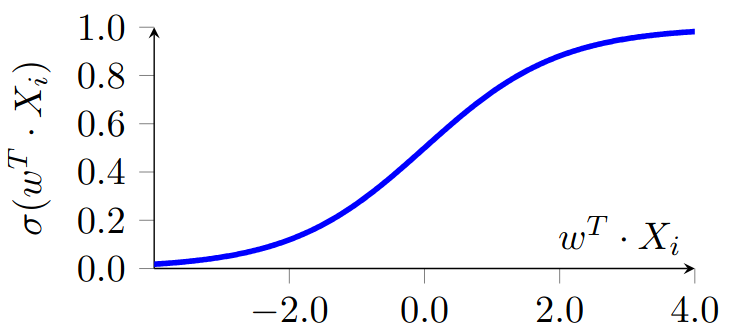
\includegraphics[width=0.4\textwidth]{images/sigmoid.png}
    \caption{Sigmoid function}
    \label{fig:sigmoid_function}
\end{figure}

During training, we want to find the best $w$ that minimize the error on the training set. The error is computed with the \emph{cross-entropy loss function}:
\begin{equation}
    \mathcal{L}(w) = -\frac{1}{N}\sum_{i=1}^{N} \Big[ Y_i \log(\mathbb{F}(X_i,w)) + (1-Y_i)\log(1-\mathbb{F}(X_i,w)) \Big]
\end{equation}

\subsection{Gradient Descent}
To minimize the loss function, we can use the \emph{Gradient Descent} algorithm. The idea is to compute the gradient of the loss function with respect to the weights, and then update the weights in the opposite direction of the gradient. If we considere a function $f(\theta)$, the gradient descent update can be expresses  as:
\begin{equation}
    \theta_j := \theta_j - \alpha \, \frac{\partial}{\partial \theta_j} f(\theta) \text{ ,for all parameter} \theta_j
\end{equation}
Where:
\begin{compactitemize}
    \item $\theta_j$ is the $j$-th parameter of the model;
    \item $\alpha$ is the \emph{learning rate}, a small positive value that controls the step size of the update;
    \item $\frac{\partial}{\partial \theta_j} f(\theta)$ is the partial derivative of the function with respect to the $j$-th parameter.
\end{compactitemize}


\begin{figure}[H]
    \centering
    \begin{minipage}{0.45\textwidth}
        \centering
        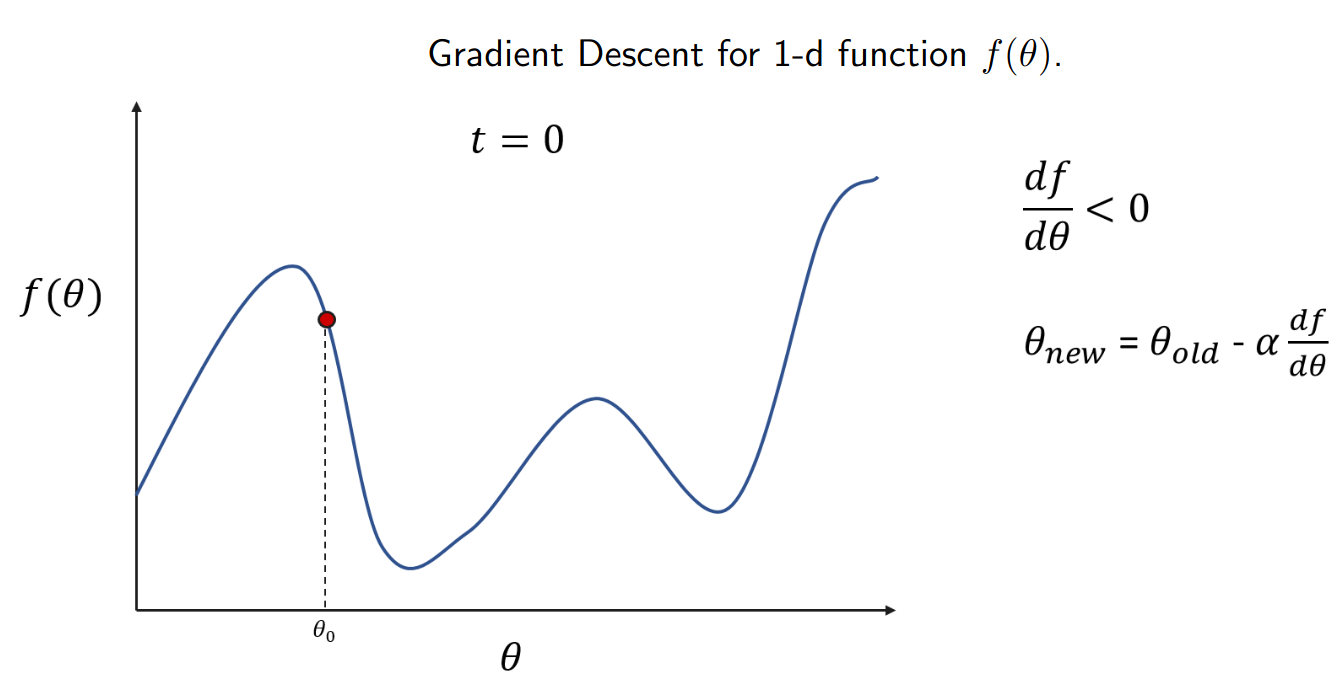
\includegraphics[width=\textwidth]{images/GD_start.png}
        \caption{Gradient Descent Start}
        \label{fig:Gradient_Descent_Start}
    \end{minipage}
    \hfill
    \begin{minipage}{0.45\textwidth}
        \centering
        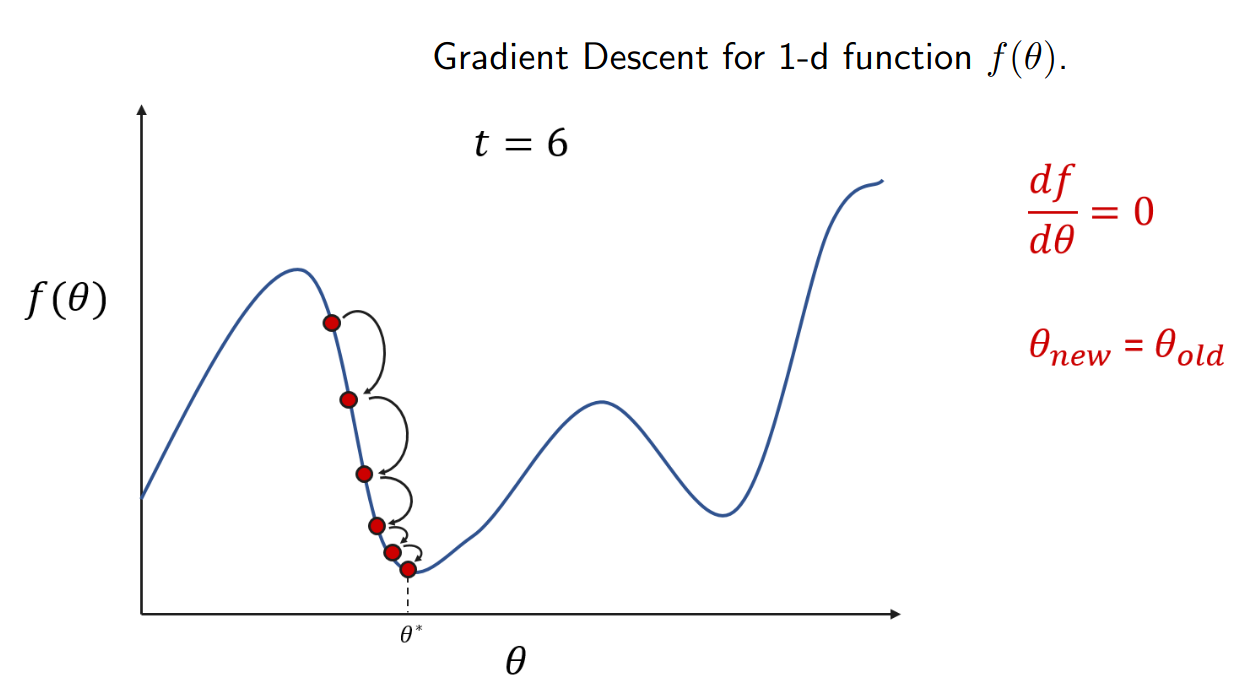
\includegraphics[width=\textwidth]{images/GD_end.png}
        \caption{Gradient Descent End}
        \label{fig:Gradient_Descent_End}
    \end{minipage}
    \label{fig:Gradient_Descent}
\end{figure}

Choosing the right learning rate $\alpha$ is essential to correctly proceed towards the minimum. Astep too small could lead to an extremely slow convergence. If the step is too big, theoptimizer could overshoot the minimum or even diverge.

\begin{figure}[H]
    \centering
    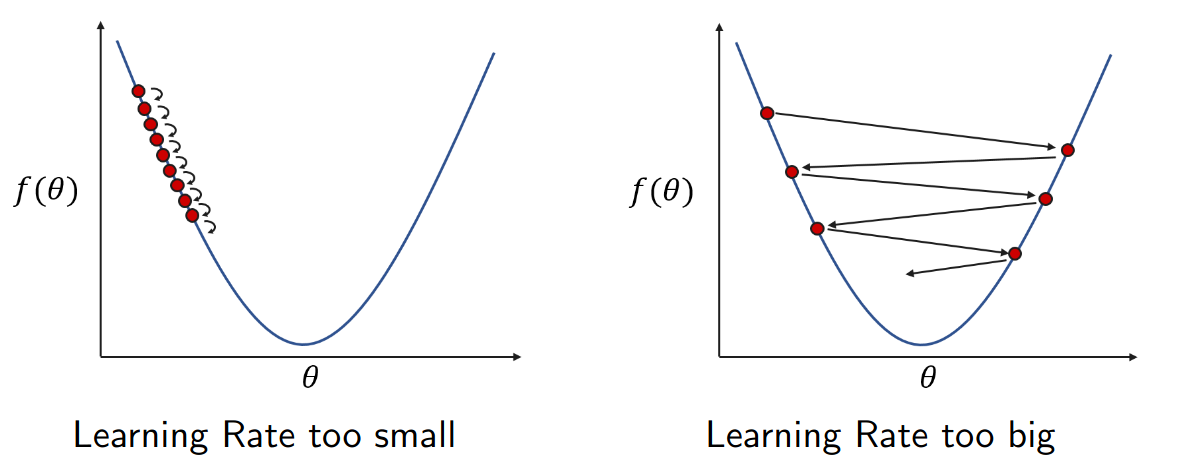
\includegraphics[width=0.8\textwidth]{images/LR.png}
    \caption{Learning Rate effect}
    \label{fig:Learning_Rate_effect}
\end{figure}

Turns out that if the function is convex, gradient descent will converge to the global minimum. For non-convex functions, it may converge to local minima.

\begin{figure}[H]
    \centering
    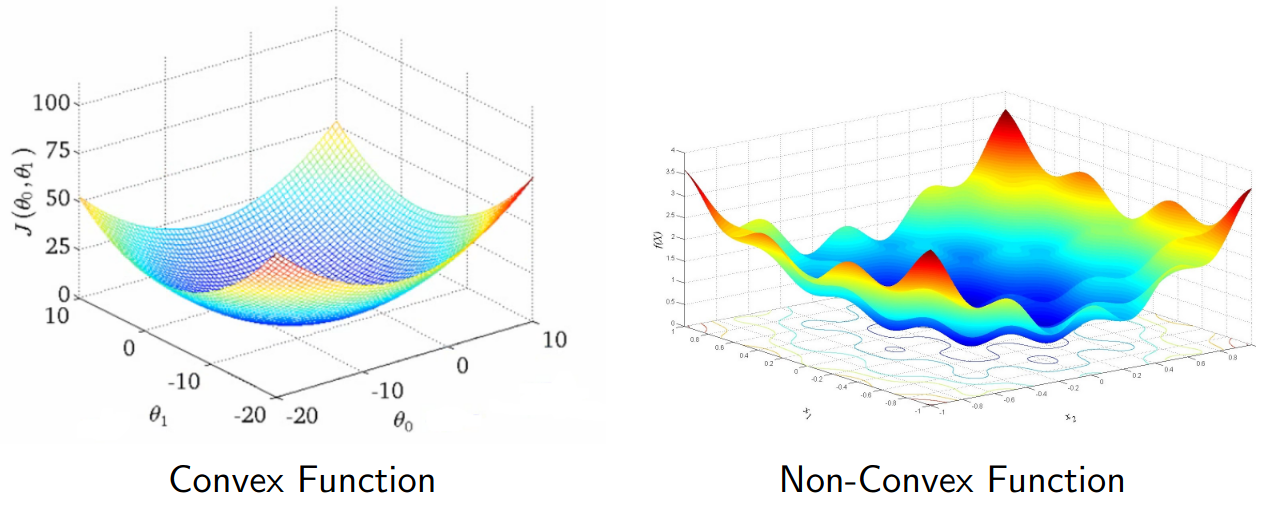
\includegraphics[width=0.8\textwidth]{images/convex_or_no.png}
    \caption{Convex or not Convex function}
    \label{fig:Convex_or_not_Convex_function}
\end{figure}

\textbf{Notes:} If we stop in a local minimum, we are not figure out with the basic GD. There are some techniques that can try to avoid or escape from local minima, like adding noise to the gradient or using momentum.

\subsection{Mathematical explanation of the weight update}
Back to our logistic regression, we want to compute the gradient of the loss function with respect to the weights. In the first we simplify the loss function:
\begin{equation}
    \begin{aligned}
    L(w) &= -\frac{1}{N} \sum_{i=1}^{N} \Big[ Y_i \log(F(X_i, w)) + (1 - Y_i) \log(1 - F(X_i, w)) \Big] \\
         &= -\frac{1}{N} \sum_{i=1}^{N} \Bigg[ 
                Y_i \log \left( \frac{e^{w^T X_i}}{1 + e^{w^T X_i}} \right) 
              + (1 - Y_i) \log \left( \frac{1}{1 + e^{w^T X_i}} \right) 
            \Bigg] \\
         &= -\frac{1}{N} \sum_{i=1}^{N} \Big[ 
                Y_i (w^T X_i) - Y_i \log(1 + e^{w^T X_i}) 
              + (Y_i - 1) \log(1 + e^{w^T X_i}) 
            \Big] \\
         &= -\frac{1}{N} \sum_{i=1}^{N} \Big[ 
                Y_i (w^T X_i) - \log(1 + e^{w^T X_i}) 
            \Big]
    \end{aligned}
\end{equation}
Now we compute the partial derivative with respect to $w_j$:
\begin{equation}
    \begin{aligned}
    \frac{\partial L(w)}{\partial w_j} 
    &= -\frac{1}{N} \sum_{i=1}^{N} \Big[ Y_i x_i^{(j)} - \frac{e^{w^T X_i}}{1 + e^{w^T X_i}} x_i^{(j)} \Big] \\
    &= -\frac{1}{N} \sum_{i=1}^{N} \Big[ \big( Y_i - \frac{e^{w^T X_i}}{1 + e^{w^T X_i}} \big) x_i^{(j)} \Big] \\
    &= -\frac{1}{N} \sum_{i=1}^{N} \Big[ \big( Y_i - F(X_i, w) \big) x_i^{(j)} \Big]
    \end{aligned}
\end{equation}
Now we can form the gradient vector and update the weights:
\begin{equation}
    \frac{\partial L(w)}{\partial w} =
    \begin{bmatrix}
    \frac{\partial L(w)}{\partial w_1} \\
    \frac{\partial L(w)}{\partial w_2} \\
    \vdots \\
    \frac{\partial L(w)}{\partial w_m}
    \end{bmatrix}
    =
    -\frac{1}{N}
    \begin{bmatrix}
    \sum_{i=1}^{N} \big(Y_i - F(X_i, w)\big) x_i^{(1)} \\
    \sum_{i=1}^{N} \big(Y_i - F(X_i, w)\big) x_i^{(2)} \\
    \vdots \\
    \sum_{i=1}^{N} \big(Y_i - F(X_i, w)\big) x_i^{(m)}
    \end{bmatrix}
    =
    -\frac{X^T \cdot (Y - F(X, w))}{N}
    \end{equation}

\textbf{Note:} Each row of the matrix is a number.

In the end we update weights with the following rule:
\begin{equation}
    w \gets w - \alpha \frac{\partial L(w)}{\partial w}
\end{equation}


\section{Optimizers}
Gradient descent is often used in machine learning to minimize a cost function, usually also called objective or loss function and denoted $L()$ or $J()$.
The cost function depends on the model’s parameters and serves as a proxy for evaluating the
model's performance. Generally speaking, in this framework minimizing the cost equals to
maximizing the effectiveness of the model.

\subsection{Stochastic Gradient Descent (SGD)}
In principle, to perform a single update step, you should run through all your training examples. This is known as \textbf{batch gradient descent}.
A different strategy is \textbf{minibatch stochastic gradient descent}. In this case, only a small subset of the training dataset is considered at each update step.
In the extreme case in which only a random example of the training set is considered to perform the update step, we talk of \textbf{stochastic gradient descent}.
This methods is typycally called vanilla SGD, and not often used in practice. 

\subsection{Advanced Optimizer}
The advanced optmizer are typycally characterized by the presence of two elements:
\begin{compactitemize}
    \item \textbf{Momentum}: using an exponentially weighted moving average of past gradients to smooth out the trajectory of the optimization, allowing faster convergence and reducing oscillations.
    \item \textbf{Adaptive Learning Rate}: scaling each parameter's learning rate by running average of the magnitude of the past gradients.
\end{compactitemize}

\begin{figure}[H]
    \centering
    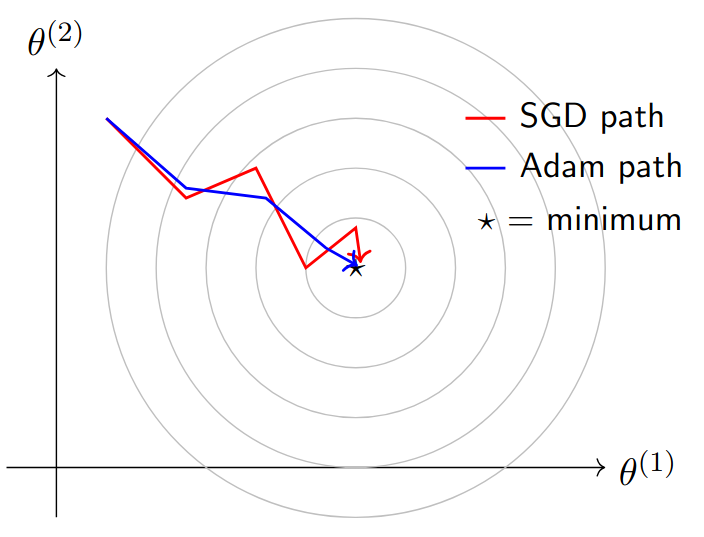
\includegraphics[width=0.5\textwidth]{images/ADAM.png}
    \caption{Advanced Optimizer}
    \label{fig:Advanced_Optimizer}
\end{figure}

\subsection{ADAM}
ADAM (short for Adaptive Moment Estimation) is an optimization algorithm that combines the benefits of both Momentum and RMSProp. It computes adaptive learning rates for each parameter by maintaining running averages of both the gradients and their squares.
The ADAM algorithm can be summarized as follows:
\begin{align}
    g_t &= \frac{\partial L}{\partial \theta_t} && \text{Gradient at step } t \\
    m_t &= \beta_1 m_{t-1} + (1 - \beta_1) g_t && \text{First moment (mean) estimate} \\
    v_t &= \beta_2 v_{t-1} + (1 - \beta_2) g_t^2 && \text{Second moment (variance) estimate} \\
    \hat{m}_t &= \frac{m_t}{1 - \beta_1^t} && \text{Bias-corrected first moment} \\
    \hat{v}_t &= \frac{v_t}{1 - \beta_2^t} && \text{Bias-corrected second moment} \\
    \theta_{t+1} &= \theta_t - \alpha \frac{\hat{m}_t}{\sqrt{\hat{v}_t} + \epsilon} && \text{Weight update}
\end{align}
\textbf{Bias correction} prevents the moment estimates from being biased toward zero, as both are initialized at zero, helping early-stage stability.\\
Typical default values for the hyperparameters are:
\begin{compactitemize}
    \item $\beta_1 = 0.9$: controls the decay rate of the moving average of the first moment (mean).
    \item $\beta_2 = 0.999$: controls the decay rate of the moving average of the second moment (variance).
    \item $\epsilon = 10^{-8}$: a small constant added to the denominator to prevent division by zero.
    \item $\alpha$: learning rate, typically set to $0.001$.
\end{compactitemize}

Let's summarize the main advantages and disadvantages of ADAM:\\
ADAM advanrages:
\begin{compactitemize}
    \item Works well out-of-the-box with minimal tuning.
    \item Handles noisy and sparse gradients effectively.
    \item Fast convergence in many pratical problems.
\end{compactitemize}
ADAM disadvantages:
\begin{compactitemize}
    \item May sometimes lead to worse generalization than SGD with momentum.
    \item Extra memory cost for moment estimates $(m_t,v_t)$.
\end{compactitemize}

    
